\def\colegio{Colegio Latinoamericano de Integración}
\def\titulo{Guía}
\def\subtitulo{Teorema de Pitágoras}
\def\curso{Octavo Básico}
\documentclass[sin nombre,con autor]{plantilla-evaluacion-v1}

\begin{document}

\tcbsidebyside[title=Definición,
sidebyside adapt=left,fonttitle=\bfseries\sffamily\scshape,center title,drop lifted shadow,
colback=white,before skip=15pt]{%
\begin{tikzpicture}[line width=1pt,scale=0.6]
  \draw (0,0) -- (0:3) coordinate (B) -- (90:4) coordinate (C)
  -- cycle coordinate (A);
  \draw (0,0) -- (0:10pt) -- ([turn]90:10pt) -- ([turn]90:10pt);

  \draw [decorate, decoration={calligraphic brace,mirror,raise=5pt,amplitude=5pt},
        line width=1pt] (A) -- (B) node [midway,below,yshift=-10pt] {$b$};
  \draw [decorate, decoration={calligraphic brace,mirror,raise=5pt,amplitude=5pt},
        line width=1pt] (B) -- (C) node [midway,above right,xshift=7pt,yshift=5pt] {$c$};
  \draw [decorate, decoration={calligraphic brace,mirror,raise=5pt,amplitude=5pt},
        line width=1pt] (C) -- (A) node [midway,left,xshift=-10pt] {$a$};

\end{tikzpicture}
}{%
Para un triángulo rectángulo, las suma de los catetos al cuadrado es igual a la hipotenusa
al cuadrado. Es decir:
\begin{equation*}
  a^2 + b^2 = c^2.
\end{equation*}
}

\section*{Ejercicios}

Calcula la medida faltante en cada caso.
\begin{preguntas}(2)
  \pregunta
  \begin{tcolorbox}[blankest,height=2.5cm]
    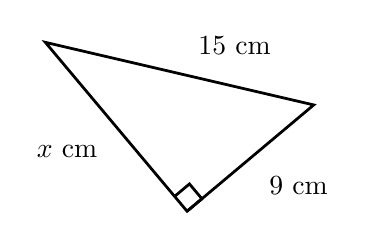
\begin{tikzpicture}[baseline=(current bounding box.north),line width=1pt,scale=0.7,rotate=40]
        \draw (0,0)
        -- (0:3) node[midway,below right=3pt] {$9$ cm}
        -- (90:4) node[midway,above right=3pt] {$15$ cm}
        -- cycle node [midway,below left=3pt] {$x$ cm};
        \draw (0,0) -- (0:10pt) -- ([turn]90:10pt) -- ([turn]90:10pt);
    \end{tikzpicture}
  \end{tcolorbox}
  \begin{malla}[height=4cm]
  \end{malla}

  \pregunta
  \begin{tcolorbox}[blankest,height=2.5cm]
    \begin{tikzpicture}[baseline=(current bounding box.north),line width=1pt,scale=0.7]
      \path[name path=lineaA] (60:3) -- ([turn]-90:6);
      \path[name path=lineaB] (0,0) -- (0:10);
      \draw[name intersections={of=lineaA and lineaB,by=x}] (0,0)
      -- (60:3) node [midway,above left=3pt] {$9$ cm}
      -- (x) node [midway,above right=3pt] {$13$ cm}
      -- cycle node [midway,below=3pt] {$y$ cm};
      \draw (60:3) -- ([turn]-90:10pt) -- ([turn]-90:10pt) -- ([turn]-90:10pt);
    \end{tikzpicture}
  \end{tcolorbox}
  \begin{malla}[height=4cm]
  \end{malla}

  \pregunta
    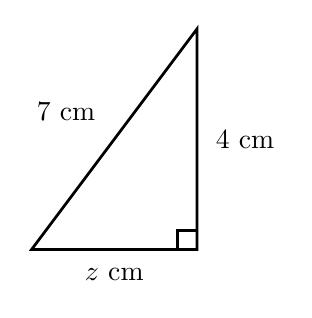
\begin{tikzpicture}[baseline=(current bounding box.north),
      line width=1pt,scale=0.7]
      \draw (0,0)
      -- (0:3) node[midway,below=3pt] {$z$ cm}
      -- ([turn]90:4) node[midway,right=3pt] {$4$ cm}
      -- cycle node[midway,above left=3pt] {$7$ cm};

      \draw (0:3) -- ([turn]90:10pt) -- ([turn]90:10pt) -- ([turn]90:10pt);

  \end{tikzpicture}
  \begin{malla}[height=4cm]
  \end{malla}

\end{preguntas}

Comprueba si los siguientes números forman un trío pitagórico.
\begin{preguntas}(2)
  \pregunta 7; 24 y 25. \\
  \begin{vertical}
    \alternativa Es pitagórico
    \alternativa No es pitagórico
  \end{vertical}
  \begin{malla}[height=3cm]
  \end{malla}
  \pregunta 10; 24 y 36. \\
  \begin{vertical}
    \alternativa Es pitagórico
    \alternativa No es pitagórico
  \end{vertical}
  \begin{malla}[height=3cm]
  \end{malla}
  \pregunta 17; 19 y 26. \\
  \begin{vertical}
    \alternativa Es pitagórico
    \alternativa No es pitagórico
  \end{vertical}
  \begin{malla}[height=3cm]
  \end{malla}
  \pregunta 1,8; 2,4 y 3. \\
  \begin{vertical}
    \alternativa Es pitagórico
    \alternativa No es pitagórico
  \end{vertical}
  \begin{malla}[height=3cm]
  \end{malla}
\end{preguntas}

Calcula el perímetro de las siguientes figuras.
\begin{preguntas}(1)
  \pregunta
  \tcbsidebyside[blanker,sidebyside adapt=left]{%
  \begin{tikzpicture}[line width=1pt,baseline=(current bounding box.north)]
    \draw (0,0)
    -- (50:3) coordinate (A)
    -- (0:5) coordinate (B)
    -- cycle coordinate (C);
    \draw [decorate, decoration={calligraphic brace,raise=5pt,amplitude=5pt},
          line width=1pt] (A) -- (B) node [midway,above right,yshift=10pt] {$26$ cm};
    \coordinate (D) at (A |- 0,0);
    \draw[dashed] (A) -- (D);
    \draw (D) -- ([turn]180:10pt) -- ([turn]-90:10pt) -- ([turn]-90:10pt) -- ([turn]-90:10pt);
    \draw [decorate, decoration={calligraphic brace,mirror,raise=5pt,amplitude=5pt},
    line width=1pt] (C) -- (D) node [midway,below,yshift=-10pt] {$7$ cm};
    \draw [decorate, decoration={calligraphic brace,raise=5pt,amplitude=5pt},
    line width=1pt] (C) -- (C |- A) node [midway,left,xshift=-10pt] {$24$ cm};
  \end{tikzpicture}
  }{%
  \begin{malla}[height=4.5cm]
  \end{malla}
  }

  \pregunta
  \tcbsidebyside[blanker,sidebyside adapt=left]{%
  \begin{tikzpicture}[line width=1pt,baseline=(current bounding box.north)]
    \draw (0,0) coordinate (A)
    -- (5,0) coordinate (B)
    -- (5,2.5) coordinate (C)
    -- (0,2.5)
    -- cycle;
    \draw (0,0) -- (0:10pt) -- ([turn]90:10pt) -- ([turn]90:10pt) -- ([turn]90:10pt);
    \draw (B) --+ (90:10pt) -- ([turn]90:10pt) -- ([turn]90:10pt) -- ([turn]90:10pt);
    \draw (C) --+ (180:10pt) -- ([turn]90:10pt) -- ([turn]90:10pt) -- ([turn]90:10pt);
    \draw (0,2.5) --+ (270:10pt) -- ([turn]90:10pt) -- ([turn]90:10pt) -- ([turn]90:10pt);

    \draw [decorate, decoration={calligraphic brace,mirror,raise=5pt,amplitude=5pt},
    line width=1pt] (B) -- (C) node [midway,right,xshift=10pt] {$8$ cm};
    \draw[dashed] (A) -- (C) node [midway,above,sloped] {$17$ cm};
  \end{tikzpicture}
  }{%
  \begin{malla}[height=4.5cm]
  \end{malla}
  }
\end{preguntas}


\end{document}

